\documentclass[11pt,a4paper]{article}
\usepackage[margin=2.2cm]{geometry}
\usepackage{amsmath,amssymb,bm}
\usepackage{graphicx,float,booktabs,caption,subcaption}
\usepackage{xcolor}
\usepackage{listings}
\usepackage{tikz}
\usetikzlibrary{shapes.geometric,arrows.meta,positioning,calc}
\usepackage[colorlinks=true,linkcolor=blue!50!black,urlcolor=blue!50!black,citecolor=blue!50!black]{hyperref}
\usepackage{fancyhdr}
\pagestyle{fancy}\fancyhf{}\lhead{\small Karthick J (OE23S018), IIT Madras}\rhead{\small\leftmark}\cfoot{\thepage}
\definecolor{codebg}{rgb}{0.97,0.97,0.97}
\lstset{basicstyle=\ttfamily\scriptsize,backgroundcolor=\color{codebg},frame=single,breaklines=true,
 keywordstyle=\color{blue!60!black}\bfseries,commentstyle=\color{green!40!black},stringstyle=\color{red!50!black},
 numbers=left,numberstyle=\tiny\color{gray},showstringspaces=false,tabsize=4,columns=fullflexible,
 literate={²}{{$^2$}}1 {³}{{$^3$}}1 {°}{{$^\circ$}}1 {Δ}{{$\Delta$}}1 {ρ}{{$\rho$}}1 {μ}{{$\mu$}}1 {ω}{{$\omega$}}1 {ψ}{{$\psi$}}1 {α}{{$\alpha$}}1 {ν}{{$\nu$}}1 {τ}{{$\tau$}}1 {–}{{-}}1 {—}{{-}}1 {’}{{'}}1 {“}{{"}}1 {”}{{"}}1 {→}{{$\to$}}1 {≤}{{$\le$}}1 {≥}{{$\ge$}}1 {×}{{$\times$}}1 {±}{{$\pm$}}1 {·}{{$\cdot$}}1 {∂}{{$\partial$}}1 {∇}{{$\nabla$}}1 {γ}{{$\gamma$}}1 {ε}{{$\varepsilon$}}1 {μ}{{$\mu$}}1 {├}{{+}}1 {─}{{-}}1 {│}{{|}}1 {▶}{{>}}1 {▼}{{v}}1 {┌}{{+}}1 {┐}{{+}}1 {└}{{+}}1 {┘}{{+}}1 {┬}{{+}}1 {┴}{{+}}1}
\tikzset{
 startstop/.style={rectangle,rounded corners=6pt,minimum width=3.2cm,minimum height=0.8cm,text centered,draw=black,fill=red!12,font=\small},
 process/.style={rectangle,minimum width=4.6cm,minimum height=0.8cm,text centered,text width=5.6cm,draw=black,fill=blue!8,font=\small},
 decision/.style={diamond,aspect=2.6,text centered,text width=3.2cm,draw=black,fill=green!12,font=\small,inner sep=1pt},
 io/.style={trapezium,trapezium left angle=72,trapezium right angle=108,minimum width=3.6cm,minimum height=0.8cm,text centered,text width=4.6cm,draw=black,fill=orange!15,font=\small},
 arrow/.style={thick,-{Stealth[length=2.5mm]}}}
\setlength{\parskip}{4pt}\setlength{\parindent}{0pt}

\title{\textbf{2-D Steady-State Heat Conduction in a Rectangular Plate}\\[2pt]\large Point, Line, SOR and ADI Iterative Solvers for the Laplace Equation in C\\[2pt]\normalsize Course Project 6 -- AM5630 Foundation of Computational Fluid Dynamics (Jul--Nov 2024)}
\author{Karthick J (OE23S018)\\Department of Ocean Engineering, IIT Madras\\Faculty: Prof.\ Arul Prakash}
\date{Revised report, October 2026}
\begin{document}\maketitle
\begin{abstract}
The steady temperature field in a $1\times2$ plate with a hot bottom wall ($100^\circ$C) and the other walls at $30^\circ$C is computed on a $21\times41$ grid with six stationary iterative methods: point Gauss--Seidel (PGS), line Gauss--Seidel (LGS), point and line successive over-relaxation (PSOR, LSOR), and alternating-direction implicit iteration (ADI) without and with relaxation. A review of the original C codes showed that the line and ADI variants never solved a tridiagonal system, that the ``ADI with relaxation'' update converged to a non-physical fixed point ($T\approx0^\circ$C in the interior) and that the heat-transfer routine integrated temperature rather than heat flux. After correction (Thomas-algorithm line solves, a consistent relaxation formula and Fourier's-law flux) all six solvers converge to the direct sparse solution of the same discrete system. LSOR and relaxed ADI are the most efficient (69 and 37 iterations at $\omega=1.5$, 41 and 21 at their optimum $\omega\approx1.7$--$1.75$), in agreement with the theoretical optimum $\omega_{opt}=1.78$ for PSOR. The discrete heat input through the bottom wall is $Q=12.81$~kW per metre depth on the $21\times41$ grid and closes the energy balance exactly; it grows logarithmically under refinement because of the temperature discontinuity at the bottom corners, while the interior temperature converges at second order.
\end{abstract}
\tableofcontents\newpage

\section{Problem definition}
\begin{figure}[H]\centering
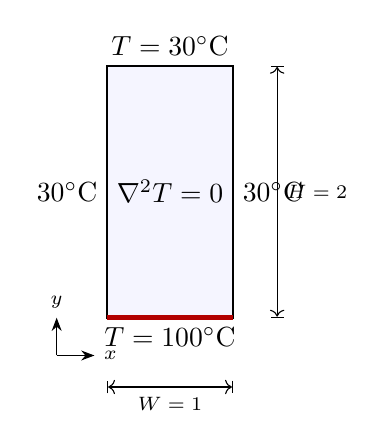
\begin{tikzpicture}[scale=1.6]
\draw[thick,fill=blue!4](0,0)rectangle(1,2);
\draw[line width=2pt,red!70!black](0,0)--(1,0); \node[below] at (0.5,0){$T=100^\circ$C};
\node[above] at (0.5,2){$T=30^\circ$C}; \node[left] at (0,1){$30^\circ$C}; \node[right] at (1,1){$30^\circ$C};
\draw[-{Stealth}](-0.4,-0.3)--(-0.1,-0.3)node[right,font=\scriptsize]{$x$}; \draw[-{Stealth}](-0.4,-0.3)--(-0.4,0)node[above,font=\scriptsize]{$y$};
\node at (0.5,1){$\nabla^2T=0$}; \draw[|<->|](0,-0.55)--node[below,font=\scriptsize]{$W=1$}(1,-0.55); \draw[|<->|](1.35,0)--node[right,font=\scriptsize]{$H=2$}(1.35,2);
\end{tikzpicture}
\caption{Domain and boundary conditions; $k=50$~W/m\,K, unit depth.}\end{figure}
\begin{equation}\frac{\partial^2T}{\partial x^2}+\frac{\partial^2T}{\partial y^2}=0,\quad 0<x<1,\;0<y<2;\qquad T(x,0)=100,\;T(0,y)=T(1,y)=T(x,2)=30. \label{eq:lap}\end{equation}
Required: (a) the steady temperature contours, (b) the heat transferred across the bottom boundary, (c) the iteration counts of the six schemes. The convergence criterion of the original code, $\max_{i,j}|T^{k+1}_{ij}-T^{k}_{ij}|<0.01^\circ$C, is retained. (The original report wrote this as a sum; the code used the maximum, which is what is reported here.)

\subsection{Analytical solution}
With $\theta=(T-30)/70$, separation of variables gives
\begin{equation}
T(x,y)=30+70\sum_{n\,\mathrm{odd}}\frac{4}{n\pi}\,\sin\!\Big(\frac{n\pi x}{W}\Big)\frac{\sinh\!\big(n\pi(H-y)/W\big)}{\sinh\!\big(n\pi H/W\big)}, \label{eq:exact}
\end{equation}
evaluated with 200 odd terms in an overflow-safe exponential form. The bottom corners carry a jump from $100$ to $30^\circ$C, so $\partial T/\partial y\sim1/r$ near them and the exact heat flux integrated over the bottom wall is (logarithmically) infinite. Any finite-grid value of $Q$ is therefore grid-dependent (Section~\ref{sec:grid}).

\section{Discretisation}
With $N_x=21$, $N_y=41$ nodes, $\Delta x=\Delta y=h=0.05$ and $\beta=\Delta x/\Delta y=1$, the five-point stencil is
\begin{equation}
T_{i+1,j}+T_{i-1,j}+T_{i,j+1}+T_{i,j-1}-4T_{i,j}=0,\qquad \tau=\mathcal{O}(h^2), \label{eq:5pt}
\end{equation}
which gives the linear system $A\mathbf{T}=\mathbf{b}$ with $n=19\times39=741$ unknowns. $A$ is symmetric positive definite, weakly diagonally dominant and has the block-tridiagonal structure $A=\mathrm{tridiag}(-I,\,B,\,-I)$ with $B=\mathrm{tridiag}(-1,4,-1)$. Writing $A=D-L-U$ (diagonal, strictly lower, strictly upper parts):
\begin{table}[H]\centering\small
\begin{tabular}{lll}\toprule
Scheme & Update & Iteration matrix $G$\\\midrule
Jacobi (reference) & $\mathbf{T}^{k+1}=D^{-1}(L+U)\mathbf{T}^k+D^{-1}\mathbf{b}$ & $G_J=D^{-1}(L+U)$\\
PGS & $(D-L)\mathbf{T}^{k+1}=U\mathbf{T}^k+\mathbf{b}$ & $G_{GS}=(D-L)^{-1}U$\\
PSOR & $T^{k+1}_{ij}=(1-\omega)T^k_{ij}+\omega\,\tilde T^{GS}_{ij}$ & $G_\omega=(D-\omega L)^{-1}[(1-\omega)D+\omega U]$\\
LGS & block GS, each row solved exactly & $(D_B-L_B)^{-1}U_B$, $D_B=\mathrm{blockdiag}(B)$\\
LSOR & line solve, then relax with $\omega$ & block SOR\\
ADI & row-implicit sweep, then column-implicit sweep & product of two block-GS operators\\\bottomrule
\end{tabular}\caption{Iterative schemes.}\end{table}
For the model problem the Jacobi spectral radius is
\begin{equation}\rho_J=\tfrac12\Big[\cos\frac{\pi}{N_x-1}+\cos\frac{\pi}{N_y-1}\Big]=0.99230,\qquad \rho_{GS}=\rho_J^2=0.9847,\qquad \omega_{opt}=\frac{2}{1+\sqrt{1-\rho_J^2}}=1.780,\end{equation}
and at $\omega_{opt}$ the SOR spectral radius drops to $\omega_{opt}-1=0.78$. The number of iterations needed to reduce the error by a factor $10^{-p}$ is $\approx p\ln10/(-\ln\rho)$, so PGS should need about twice as many iterations as Jacobi and SOR an order of magnitude fewer.

\subsection{Line solves (Thomas algorithm)}
In LGS/LSOR every interior row $i$ is solved implicitly in $x$ with the neighbouring rows at their latest values:
\begin{equation}
-T_{i,j-1}+4T_{i,j}-T_{i,j+1}=T_{i-1,j}+T_{i+1,j},\qquad j=1,\dots,N_x-2, \end{equation}
a tridiagonal system solved in $\mathcal{O}(N_x)$ operations by forward elimination
$c'_k=c_k/(b_k-a_kc'_{k-1})$, $d'_k=(d_k-a_kd'_{k-1})/(b_k-a_kc'_{k-1})$ and back substitution $x_k=d'_k-c'_kx_{k+1}$. LSOR then sets $T_{ij}\leftarrow(1-\omega)T_{ij}^{old}+\omega T^{*}_{ij}$. ADI repeats the same in $y$ (columns) after the $x$ sweep, so information crosses the whole domain in both directions in every iteration.

\subsection{Heat transfer through the bottom wall}
By Fourier's law the heat entering through the bottom face (per unit depth) is
\begin{equation}
Q=-k\!\int_0^W\!\frac{\partial T}{\partial y}\Big|_{y=0}\!dx\;\approx\;k\sum_{j=1}^{N_x-2}\frac{T_{1,j}^{\,wall}-T_{2,j}}{\Delta y}\,\Delta x ,
\end{equation}
which is exactly the flux carried by the five-point stencil across the bottom faces, so the discrete energy balance $Q_{bottom}=Q_{top}+Q_{left}+Q_{right}$ closes to round-off.

\subsection{Algorithm}
\begin{figure}[H]\centering
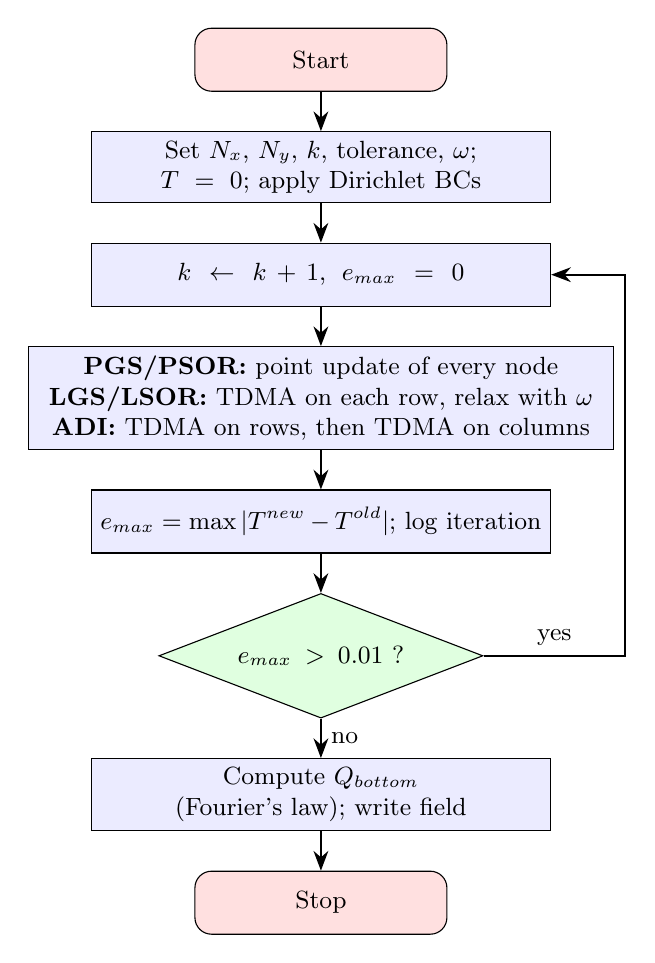
\begin{tikzpicture}[node distance=0.5cm]
\node(s)[startstop]{Start};
\node(i)[process,below=of s]{Set $N_x$, $N_y$, $k$, tolerance, $\omega$; $T=0$; apply Dirichlet BCs};
\node(it)[process,below=of i]{$k\leftarrow k+1$, \;$e_{max}=0$};
\node(sw)[process,below=of it,text width=7.2cm]{\textbf{PGS/PSOR:} point update of every node\\\textbf{LGS/LSOR:} TDMA on each row, relax with $\omega$\\\textbf{ADI:} TDMA on rows, then TDMA on columns};
\node(e)[process,below=of sw]{$e_{max}=\max|T^{new}-T^{old}|$; log iteration};
\node(d)[decision,below=of e]{$e_{max}>0.01$ ?};
\node(q)[process,below=of d]{Compute $Q_{bottom}$ (Fourier's law); write field};
\node(f)[startstop,below=of q]{Stop};
\draw[arrow](s)--(i);\draw[arrow](i)--(it);\draw[arrow](it)--(sw);\draw[arrow](sw)--(e);\draw[arrow](e)--(d);
\draw[arrow](d)--node[right,font=\small]{no}(q);\draw[arrow](q)--(f);
\draw[arrow](d.east)--node[above,font=\small]{yes}++(1.8,0)|-(it.east);
\end{tikzpicture}\caption{Common structure of the six solvers (\texttt{code/*.c}).}\end{figure}

\section{Code review and corrections}
\begin{table}[H]\centering\small
\begin{tabular}{p{2.6cm}p{6.6cm}p{6.1cm}}\toprule
File (original) & Problem & Correction\\\midrule
all six & \texttt{calculateHeatTransfer} returned $k\int T\,dx$ ($=4825$ for every scheme). This has units of W\,m$^{-1}$K$^{-1}\cdot$K$\cdot$m but is not a heat rate. & Fourier's-law flux through the bottom faces (Eq.~above).\\
\texttt{Line\_gauss\_sidel.c} & Two point-wise sweeps (along $x$, then $y$) per iteration; no implicit line solve. & TDMA on each row (true LGS).\\
\texttt{PSOR.c}, \texttt{Lsor.c} & Identical programs: two point-SOR sweeps per iteration. Neither is LSOR, and PSOR counted two sweeps as one iteration. & PSOR: one point sweep; LSOR: TDMA row solve + relaxation.\\
\texttt{ADI\_method.c} & ``Iteration level 0.5'' used as under-relaxation of point updates; no line solves. & Row TDMA then column TDMA (ADI line iteration).\\
\texttt{ADI\_method\_with\_relaxation.c} & $T=(1-\omega)T^{old}+\omega\cdot0.5\,\bar T$: the fixed point is $T=0.5\bar T$, i.e.\ the field is driven towards zero. It ``converged'' in 8 iterations to $T\approx0$--$5^\circ$C in the interior (Fig.~\ref{fig:old}). & Row and column TDMA with standard over-relaxation.\\\bottomrule
\end{tabular}\caption{Defects and corrections. Originals are in \texttt{original/code\_JulNov2024/}; the earlier Jan--May 2024 C++ versions are kept in \texttt{original/code\_JanMay2024/}.}\end{table}
Grid, boundary conditions, initial guess, tolerance, console/file output and code layout were otherwise kept. One routine, \texttt{writeFinalField}, was added to write the converged field at full precision for post-processing.

\section{Results}
\subsection{Temperature field}
\begin{figure}[H]\centering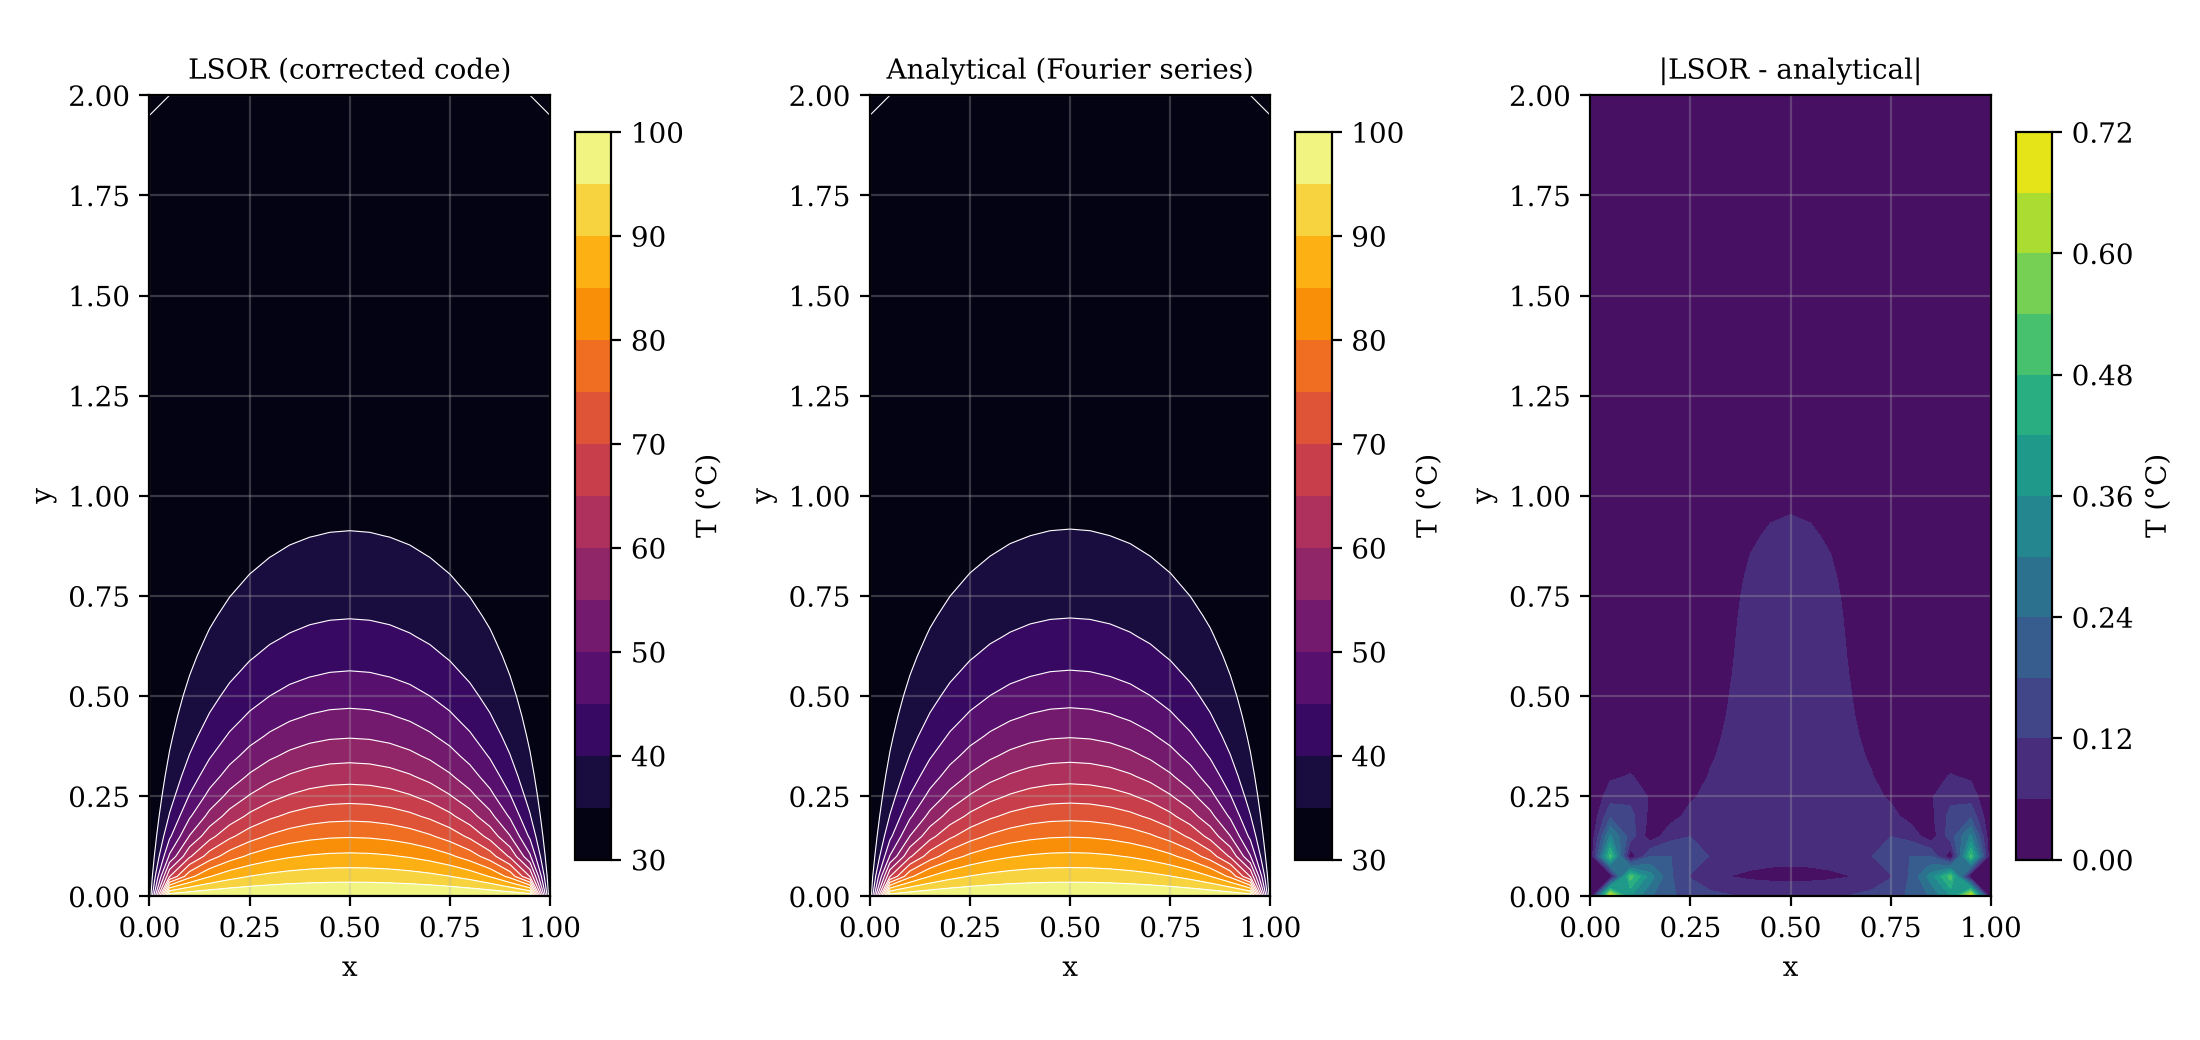
\includegraphics[width=\textwidth]{../results/fig1_temperature_contours.png}
\caption{Steady temperature (LSOR, corrected), analytical solution (\ref{eq:exact}) and their difference.}\end{figure}
Heat enters through the bottom and leaves mainly through the side walls; the isotherms are symmetric about $x=0.5$ and decay roughly as $e^{-\pi y}$, so above $y\approx1$ the plate is within $3^\circ$C of $30^\circ$C. The numerical and analytical fields agree to better than $0.1^\circ$C away from the bottom corners. The largest differences ($\le0.7^\circ$C) sit in the cells next to the corner discontinuities, where the exact solution is not smooth.

\subsection{Convergence of the iterative schemes}
\begin{figure}[H]\centering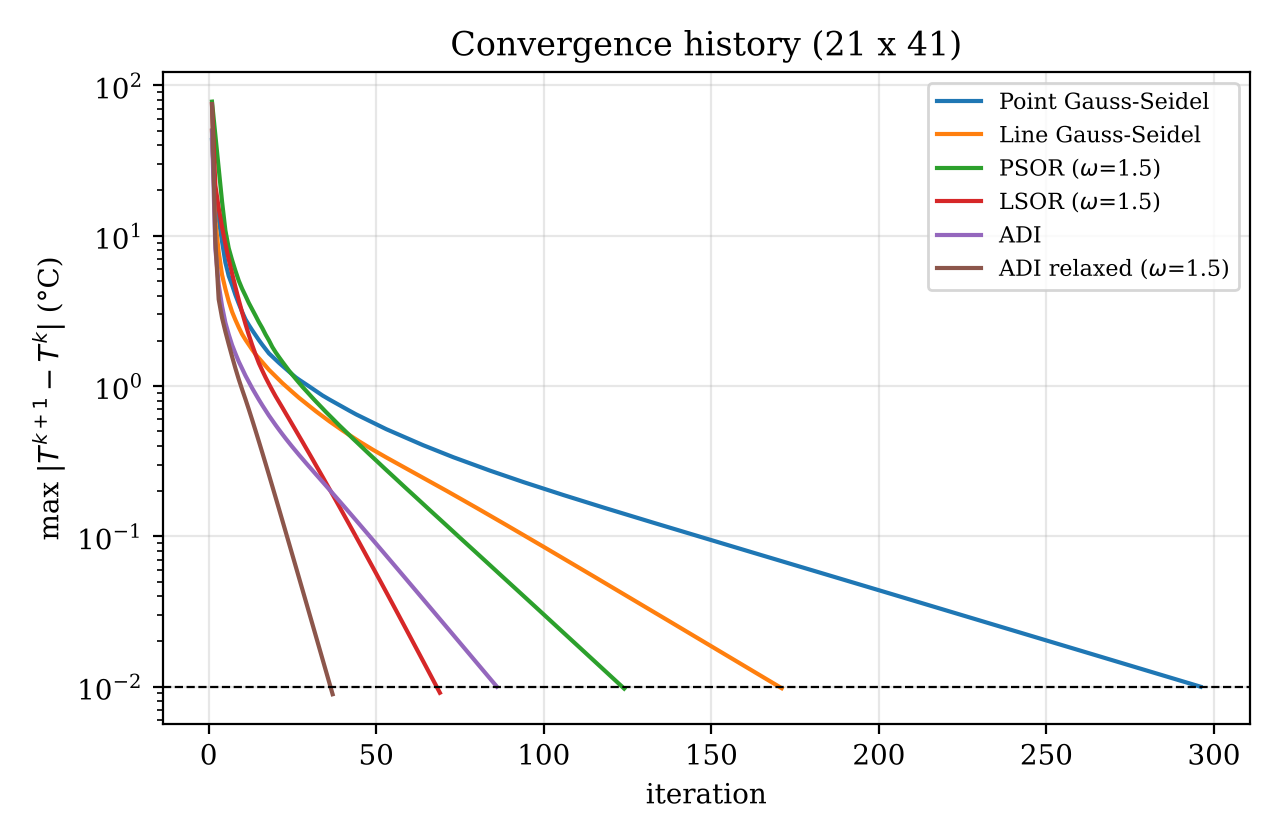
\includegraphics[width=0.72\textwidth]{../results/fig2_convergence_history.png}
\caption{Maximum change per iteration. The straight lines on the log scale are the asymptotic rates $\rho(G)$.}\end{figure}
\begin{table}[H]\centering\small
\begin{tabular}{lccccc}\toprule
Scheme & Iterations & $Q_{bottom}$ (W/m) & $\max|T-T_{direct}|$ ($^\circ$C) & Orig.\ iterations & Orig.\ ``$Q$''\\\midrule
Point Gauss--Seidel & 296 & 12\,842 & 0.64 & 296 & 4\,825\\
Line Gauss--Seidel & 171 & 12\,834 & 0.31 & 149$^*$ & 4\,825\\
PSOR ($\omega=1.5$) & 124 & 12\,820 & 0.20 & 63$^*$ & 4\,825\\
LSOR ($\omega=1.5$) & 69 & 12\,823 & 0.089 & 63$^*$ & 4\,825\\
ADI & 86 & 12\,831 & 0.31 & 336 & 4\,825\\
ADI relaxed ($\omega=1.5$) & 37 & 12\,819 & 0.081 & 8$^\dagger$ & 4\,825\\
Direct sparse solve & -- & 12\,814 & 0 & -- & --\\\bottomrule
\end{tabular}
\caption{Results on $21\times41$. $^*$Two sweeps per counted iteration. $^\dagger$Converged to a wrong field.}\label{tab:res}\end{table}
Observations:
\begin{itemize}
\item The iteration counts follow the theory: line methods couple a whole row implicitly and roughly halve the iterations of their point counterparts (LGS 171 vs PGS 296; LSOR 69 vs PSOR 124), and alternating the line direction (ADI) gains another factor of two.
\item The stopping test is on the \emph{increment}, not the error. Since $\|e^k\|\approx\|T^{k+1}-T^k\|/(1-\rho)$, a slowly converging method stops far from the solution: PGS ($\rho\approx0.985$) stops with an error of $0.64^\circ$C even though the increment is $<0.01^\circ$C. A tolerance of $0.01(1-\rho)$, or a residual-based test, should be used for accuracy-sensitive work.
\item The original iteration counts for LGS, PSOR and LSOR look smaller only because each counted iteration contained two sweeps.
\end{itemize}

\subsection{Relaxation factor}
\begin{figure}[H]\centering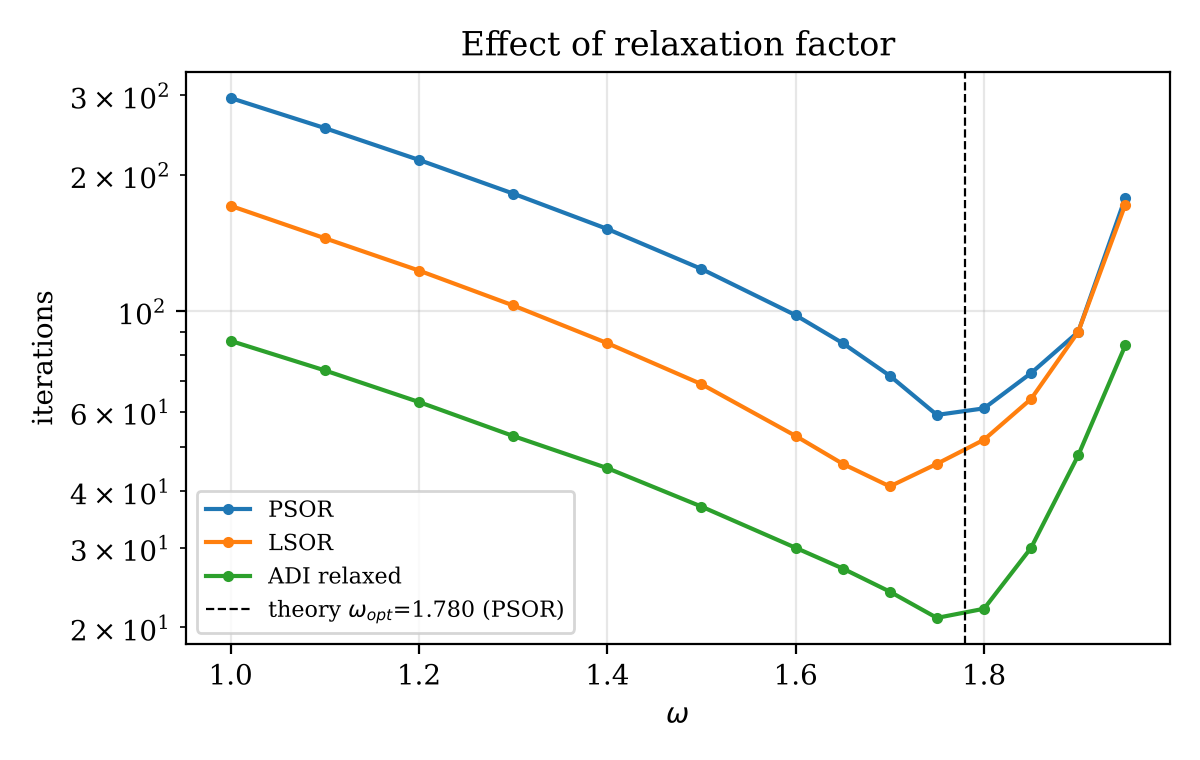
\includegraphics[width=0.66\textwidth]{../results/fig4_omega_sweep.png}
\caption{Iterations vs.\ $\omega$ (corrected PSOR, LSOR and relaxed ADI).}\end{figure}
PSOR reaches its minimum (59 iterations) at $\omega=1.75$, close to the theoretical $\omega_{opt}=1.78$; LSOR (41 at $\omega=1.70$) and relaxed ADI (21 at $\omega=1.75$) have slightly lower optima, consistent with their smaller unrelaxed spectral radii. Beyond the optimum the iteration count rises steeply as $\rho(G_\omega)=\omega-1$ grows.

\subsection{Original versus corrected code}
\begin{figure}[H]\centering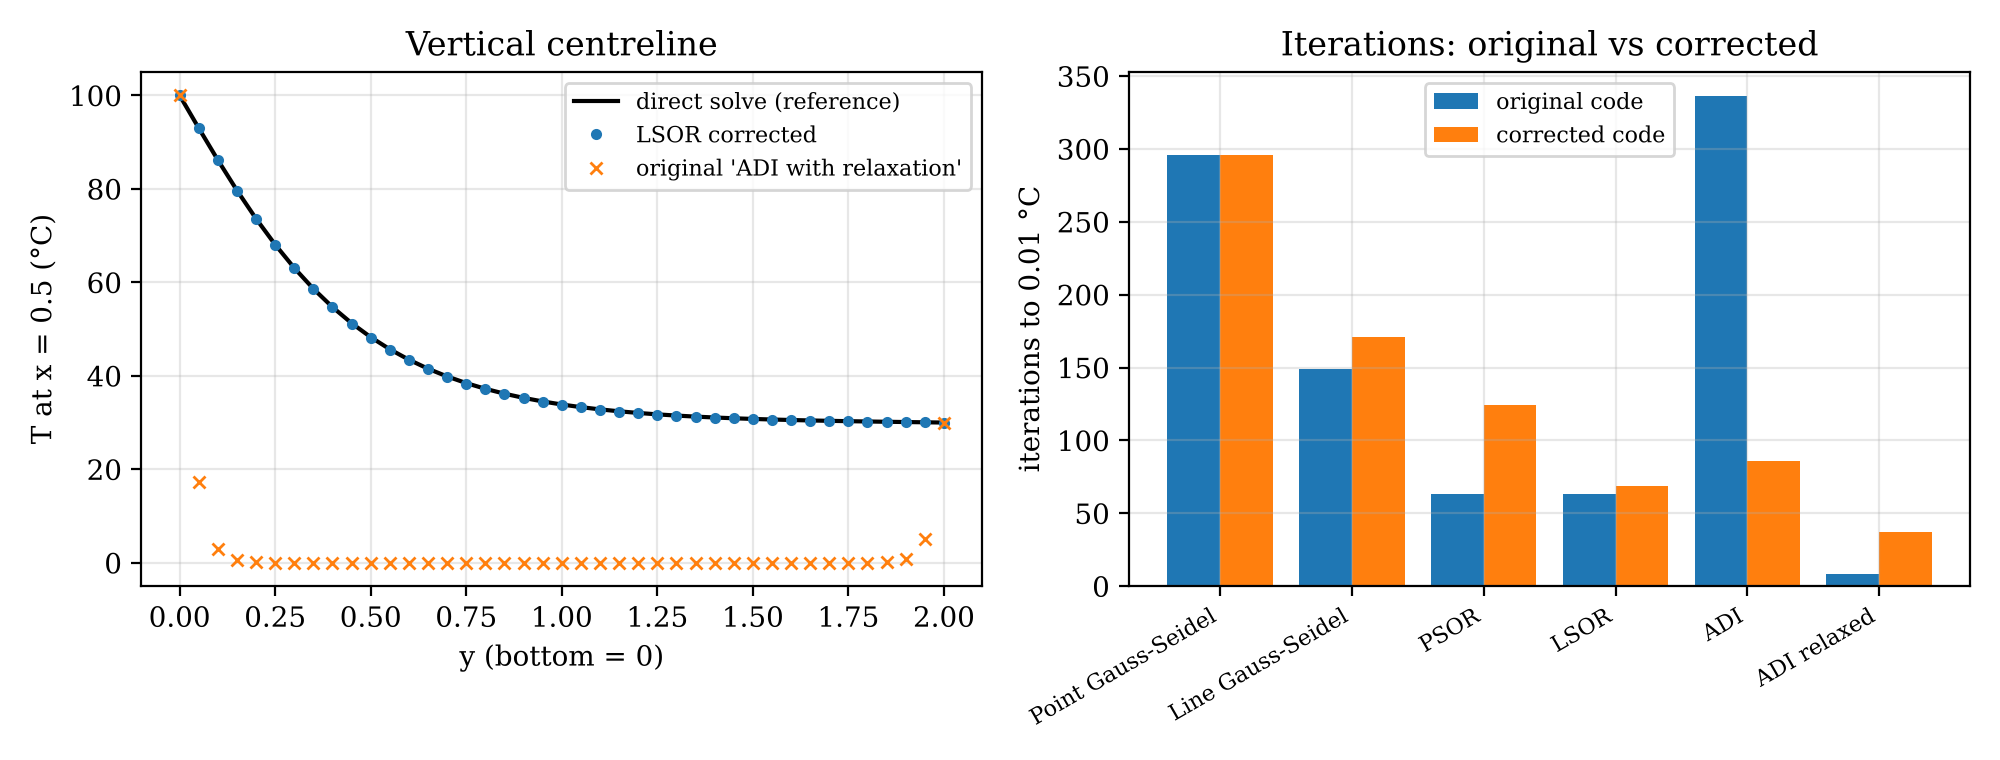
\includegraphics[width=\textwidth]{../results/fig3_original_vs_corrected.png}
\caption{Left: centreline temperature; the original ``ADI with relaxation'' result collapses to $\approx0^\circ$C. Right: iteration counts of original and corrected codes.}\label{fig:old}\end{figure}

\subsection{Heat balance and grid study}\label{sec:grid}
For the direct solution on $21\times41$: $Q_{bottom}=12\,813.6$~W/m $=Q_{left}+Q_{right}+Q_{top}=6\,390.0+6\,390.0+33.6$~W/m, so the balance closes exactly and more than 99.7\% of the heat leaves through the side walls.
\begin{figure}[H]\centering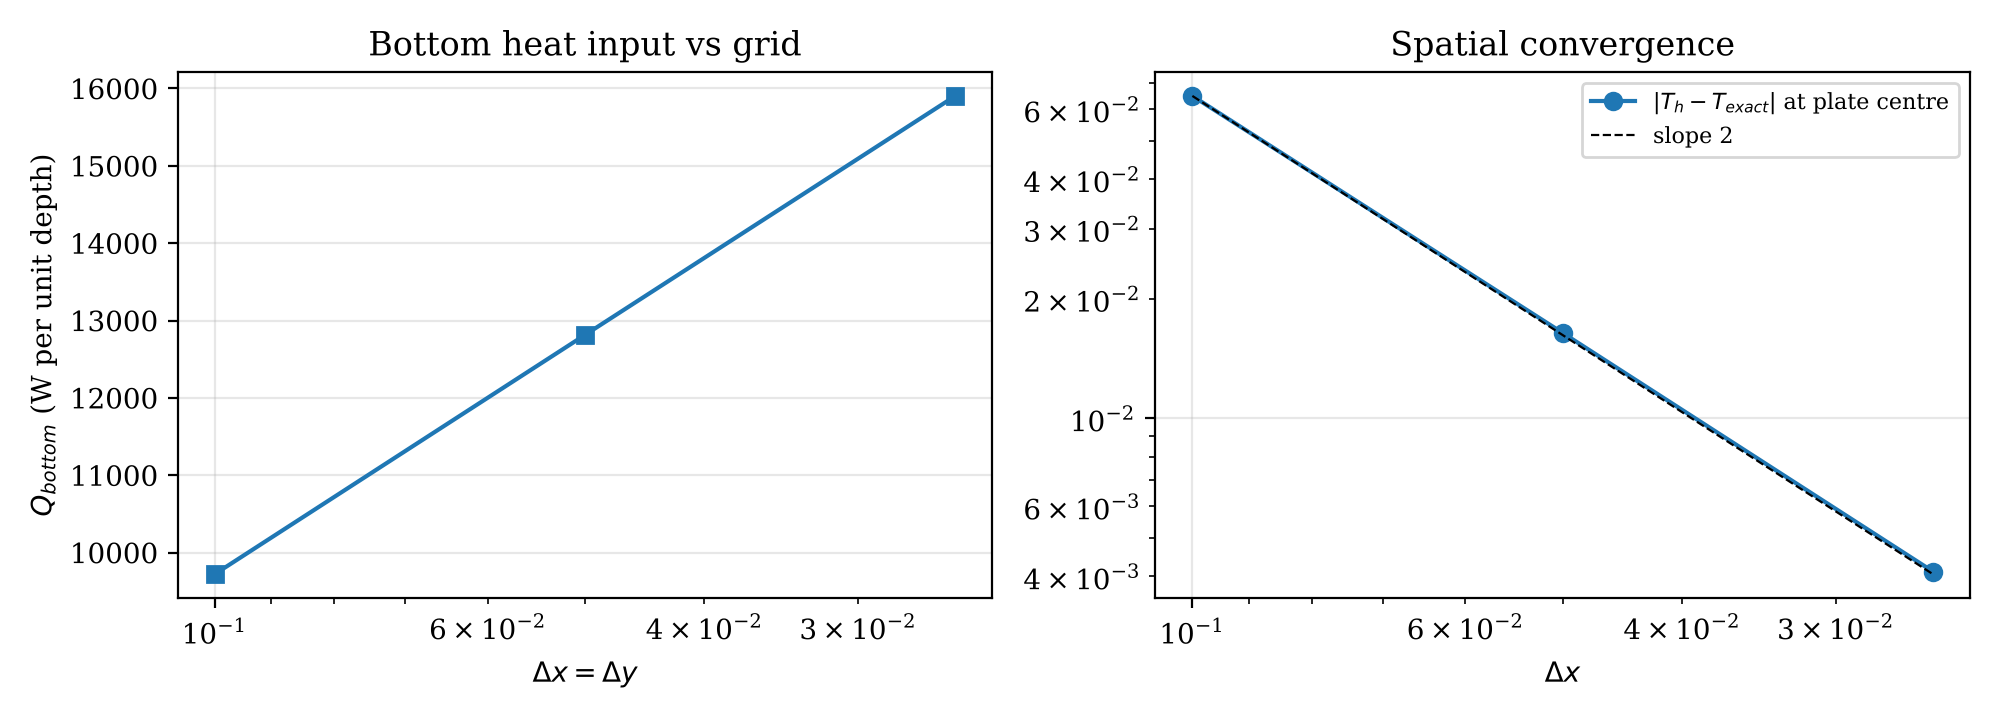
\includegraphics[width=\textwidth]{../results/fig5_grid_study.png}
\caption{Grid study with LSOR converged to $10^{-9}$: bottom heat input and centre-point error.}\end{figure}
\begin{table}[H]\centering\small\begin{tabular}{cccc}\toprule
Grid & $Q_{bottom}$ (W/m) & $T(0.5,1)$ & $|T-T_{exact}|$\\\midrule
$11\times21$ & 9\,720 & 33.9067 & $6.5\times10^{-2}$\\
$21\times41$ & 12\,814 & 33.8583 & $1.6\times10^{-2}$\\
$41\times81$ & 15\,904 & 33.8461 & $4.2\times10^{-3}$\\\bottomrule\end{tabular}\caption{Grid convergence ($T_{exact}(0.5,1)=33.8419$).}\end{table}
The plate-centre error falls by a factor of $\approx4$ per halving of $h$ (second-order accuracy). $Q_{bottom}$, by contrast, increases by an almost constant $\approx3.09$~kW/m per halving, i.e.\ $Q\propto\ln(1/h)$: this is the discrete signature of the $1/r$ flux singularity at the bottom corners. The value $12.8$~kW/m is the correct answer \emph{for the $21\times41$ grid specified in the assignment}, but it is not grid-independent.

\section{Conclusions}
\begin{itemize}
\item After correction, all six solvers converge to the direct solution of the discrete Laplace system; the temperature agrees with the analytical series to $<0.1^\circ$C away from the corners and is second-order accurate.
\item Efficiency ranking at $\omega=1.5$: relaxed ADI (37) $<$ LSOR (69) $<$ ADI (86) $<$ PSOR (124) $<$ LGS (171) $<$ PGS (296). At the optimum $\omega\approx1.7$--$1.75$ this becomes 21 / 41 / 59 iterations for relaxed ADI / LSOR / PSOR.
\item The bottom heat input is $Q=12.81$~kW per metre depth on $21\times41$, with an exactly closed energy balance; it diverges logarithmically with refinement because of the corner temperature jump.
\item The original codes contained three method-level errors (no line solves, a scaling factor that drove ``ADI with relaxation'' to a wrong solution, and a heat-transfer formula without a gradient); these were corrected without changing the problem set-up.
\end{itemize}

\section*{Reproducing the results}
\texttt{bash run.sh} compiles and runs the six corrected and six original codes, the $\omega$ sweep and the grid study, then calls \texttt{code/postprocess.py} (NumPy, SciPy, Matplotlib).

\appendix\section{Corrected source: line SOR}
\lstinputlisting[language=C]{../code/lsor.c}
\section{Corrected source: ADI with relaxation (iteration loop)}
\lstinputlisting[language=C,firstline=176]{../code/adi_relaxation.c}
\end{document}
